\section{Overview of Sensibility Testbed}\label{sec-overview}
%Here we are going to put the overview and high-level walkthrough. 
%(I'm putting the old Section 3.3 here for now. )
\jill{it sounds like the whole section is solely about default policies- 
let's maybe add in more of a general statement here on the design as a whole}
The center if \sysname is its policies. We introduce how the default
policies are designed, and the procedures to follow if default policies
become insufficient. We further descrive \sysname's design guideline 
and the resulting testbed components. We also show the testbed operation.

\subsection{A High-level Walkthrough}\label{sec-walkthrough}

\begin{figure}
\center{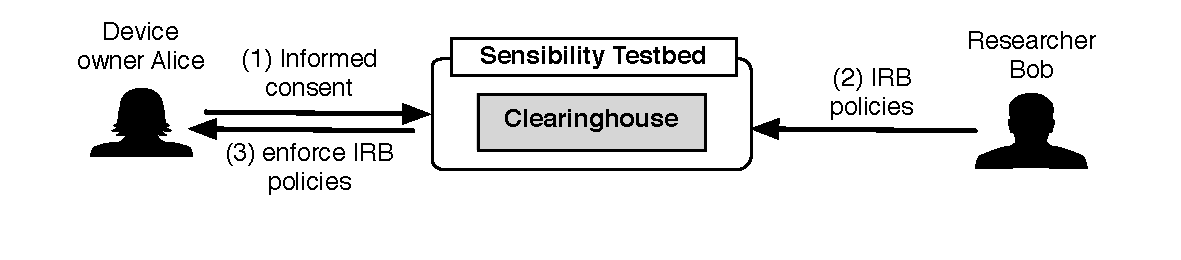
\includegraphics[width=\columnwidth]{figs/irb.pdf}}
%\vspace*{-20pt}
\caption{\small A high-level walkthrough. \label{fig-walkthrough}}
\end{figure}

The basic operation of Sensibility Testbed involves two separate 
parties: a device owner interested in participating in experiments 
and a researcher seeking to run tests on remote devices. In the 
following walk through, we assume that Alice, a device owner, participates in 
the testbed, while a researcher, Bob, runs code on Sensibility Testbed 
using Alice's smartphone, among other
devices. Let's suppose that the goal of Bob's experiment is to determine the cellular service
quality in major cities. His experiment therefore needs to obtain location information
of individual devices, their cellular service provider, network
<<<<<<< HEAD
type (3G, 4G, LTE, etc.), and signal strength. 

Alice wants to allow scientists to perform experiements using her smartphone.
She starts by installing the Sensibility Testbed app from 
the Android app store~\cite{sensibility-app}. After downloading the app, 
Alice is informed about the testbed's privacy and use policy 
in a consent form and must give consent before participating.
Any device owner, regardless of age, country, or background, can 
opt into our testbed in this manner \cappos{Is this true of pregnant women, 
children, etc.?  They are in protected groups...}, and can opt out just by 
uninstalling the app. The app will also display a list of experiments and 
each experiment's policies, so Alice can opt out of individual experiments. 
\cappos{how is this updated?  Does Alice see this before or after an 
experiment may run?  How much "lead time" does Alice get to opt-out
before the experiment happens?}
\cappos{Do you want to say something about informed consent here or
does it fit better later?}

To conduct an experiment, Bob will first provide his institution's 
IRB policies  \cappos{I don't think this is phrased correctly.  I think 
you mean to say that Bob goes through the IRB process at his institution.}
to the clearinghouse (Section~\ref{sec-ch}) and sign up for his experiment. 
\cappos{Doesn't Bob get materials from our site (via the checkboxes, etc.)
that help with his IRB process?}
The clearinghouse server helps him acquire devices, and codifies 
policies specified by Bob's IRB. After obtaining remote devices, 
Bob can perform experiments directly on the devices through 
an experiment manager (Section~\ref{sec-emt}), \cappos{I think that these 
details don't matter.  They don't know what an experiment manager, 
clearinghouse, etc.  are at this point.} using the 
credentials assigned by the clearinghouse. Such a 
protocol for research with mobile device sensors has been approved by
the IRB at New York University (IRB \# 15-10751).  \cappos{I do not understand
how this ties into the main point.  Why does Bob need to know this to
do an experiment?  If he doesn't, then this does not fit here.}

The form that Bob previously filled out on the Sensibility site is used to
enforce a technical set of restrictions for his experiment.  This means
that regardless if Bob makes an error or is malicious, his experiment is
restrited in the data it can gather.  So Bob's IRB form which requests 
access to GPS and cellular information, would result in him being blocked
from reading the roaming status despite it being tracked under the same
Android permission as the other cellular ID information.  

Note that the form has limits to the precision of data that Bob can request
for many sensors (e.g., preventing access to the raw MAC address of the device).
If Bob has a legitimate need for this data and can appropriately secure it,
Bob can request such access by also passing his locally approved request 
through NYU's IRB.  This additional check ensures not only that Bob's 
handling and access to the data is appropriate, but ensures that this does
not violate Alice's privacy and use policy with the Sensibility Testbed.
%When Bob's IRB wants to access information that is more sensitive than
%what is described in NYU IRB, \yanyan{Justin, help!}  

Once Bob's experiment has been approved and the appropriate privacy
restrictions are identified, Bob may now run his experiment on the
devices of participants like Alice.  \cappos{Is here a better place
to move the opt-out text?}.  Alice's informed consent to Sensibility Testbed
ensures that Bob does not need to individually recruit Alice to include
her smartphone's data in his study.

\cappos{Extra text.}
This work flow is shown in Figure~\ref{fig-walkthrough}. \sysname
acts as an intermediate between the device owner and researcher, 
where the device owners give their informed consent, and researchers
provide their IRB policies. As a result, the researchers do not recruit
device owners directly for each experiment, and the testbed infrastructure 
enforces the IRB policies on behalf of the researcher. \yanyan{where 
should NYU IRB lie in this figure?}

\sysname's default policies are described next.
=======
type (3G, 4G, LTE, etc.), and signal strength. Bob has obtained an IRB for gathering 
his experiment data. At the same time, Alice wants to be ensured that her privacy is 
protected according to the policies specified in Bob's IRB.

In order for Alice to participate in Sensibility Testbed as a device owner,
she starts by installing the Sensibility Testbed app from 
the Android app store~\cite{sensibility-app}. After downloading the app, 
Alice has the opportunity to select which experiments she would like to opt into, 
though at any time she can choose to opt out of any individual experiment or her 
complete participation in the testbed.

To conduct an experiment, Bob will first provide his institution's 
IRB policies to the clearinghouse (Section~\ref{sec-ch}) component of Sensibility Testbed 
and sign up for his experiment. 
The clearinghouse server helps him acquire devices and automatically codifies 
policies specified by Bob's IRB. After obtaining remote devices, 
Bob can perform experiments directly on the devices through 
an experiment manager (Section~\ref{sec-emt}), using the 
credentials assigned by the clearinghouse. The app installed on Alice's device will 
automatically enforce the IRB privacy policies on any data collected before it leaves her device and 
goes to Bob. If Bob's IRB requests that all location data is provided by subjects at 
a city-level granularity, for example, Alice's exact location will be obscured 
to the nearest city before Bob can access it. 
If Bob wishes to run a
second experiment using either the same or different IRB policies, Sensibility Testbed 
greatly simplifies this process by enabling 
him to do so without having to recruit subjects again or re-implement the 
IRB policies in his experiment code.
Such a 
protocol for research with mobile device sensors has been approved by
the IRB at New York University (IRB \# 15-10751). 

This work flow is shown in Figure~\ref{fig-walkthrough}. \jill{let's add how Bob gets the 
data from Alice's device in Figure 1} \sysname
acts as an intermediate between the device owner and researcher, 
where the device owners give their informed consent, and researchers
provide their IRB policies. 
>>>>>>> a59aa3d25f287a6b156075d6ead8886f9281b705

%Device owners like Alice participate in Sensibility Testbed by p.

%These policies restrict what and how data can be accessed by the 
%researcher. 
%into data blurring layers that are enforced on
%mobile devices. Such a process can protect device
%owners' personal information. 
%Researchers' code runs in a sandbox that isolates the code from the 
%rest of the device host system. 
%To control the execution of code, Bob uses his own 
%desktop or laptop computer to manage the 
%experiments via the experiment manager. It deploys 
%and runs experiments in sandboxes on remote devices that are 
%acquired through the clearinghouse.

%\textbf{Usage scenario 1: Smartphone owner volunteers as a testbed participant.}
%Alice downloads the Sensibility Testbed app from the Google Play 
%Store~\cite{sensibility-app}, which will install Repy and other software on her phone.
%The app displays a consent form, \yanyan{cite link} containing the testbed's 
%general usage policy. Alice must review and must agree to this 
%policy before installation. If Alice gives her consent, her device will be 
%installed with the Repy sandbox, the native Android code to 
%start or stop the sandbox, and an interface to communicate with the testbed 
%infrastructure (particularly the clearinghouse, described below). 
%By agreeing to our general usage policy, any device 
%owner, regardless of age, country, or background, need only to opt into our testbed as a
%volunteer \textit{once}, at the time of app installation. 
%%As a result, an 
%%researcher like Bob who wants to conduct an experiment 
%%%requests devices through our clearinghouse, which assigns 
%%%them devices from a set of available resources. As a result, 
%%%the researcher
%%does not need to get consent from each subject for each individual
%%experiment. \lois{is the previous sentence needed? I don't think so} 
%The testbed thus greatly simplifies the process for both the 
%device owners and experimenters. 


\begin{table*}
\scriptsize
\centering

\bgroup
\def\arraystretch{1.15}% % for table padding
\begin{tabular}{|p{1.6cm}|p{8cm}|p{4cm}|c|}
\hline
{\bf Goals\textsuperscript{*}}  & {\bf Sensor data} & {\bf Precision 
policy\textsuperscript{\dag}} & {\bf Frequency policy\textsuperscript{\dag}} \\ \hline \hline

\multirow{7}{1.7cm}{Support research projects.} & Battery status (charging/discharging), temperature, 
 technology, health (good/overheat), battery level, voltage, plug-in type. & 
 \multirow{7}{4cm}{Full precision, round-up (if numeric), or constant.} & 
 \multirow{7}{*}{N/A} \\ \cline{2-2}
 
& Bluetooth scan mode, state (enabled/disabled). & &  \\ \cline{2-2}
 
& Cellular network roaming status, SIM card status (ready/absent), 
phone status (idle/busy), signal strength. &  &  \\ \cline{2-2}

& WiFi link speed, association state, nearby routers' frequency, signal strength. & & \\ \cline{2-2}
  
& Vibrate mode, screen settings (on/off, brightness, timeout), media/ringer 
volume. & &  \\ \hline 

%%%%%%%%%%%%%%%%%%%%%%%%%%%%%%%%%%%%%%

Prevent keyloggers. & Motion sensors: accelerometer, gyroscope, magnetometer, 
orientation, ambient light. & Full precision, roundup, random rotation, or constant. & 
\multirow{2}{*}{< 100 Hz} \\ \hline 

%%%%%%%%%%%%%%%%%%%%%%%%%%%%%%%%%%%%%%

\multirow{8}{1.7cm}{Prevent locating a device.} & 
\multirow{2}{*}{Latitude, longitude, altitude.}  & Approximate to the nearest 
zipcode region, or city/state/country center. & \multirow{8}{*}{Once per 10 minutes.} \\\cline{2-3}
%& & Speed. & Round-up, or constant. & \\\cline{3-4}
& Location service provider. & Full string, or constant. & \\ \cline{2-3}

& Nearby Bluetooth device names. & Hashed device names. &  \\ \cline{2-3}

& Cellular network cell ID, neighboring cell ID(s). & Randomized ID. &  \\ \cline{2-3}
& Cellular network operator ID and name, country code, area code. & Hashed ID, names, 
and code. &  \\ \cline{2-3}

& WiFi connection information (router's SSID and MAC address). 
& \multirow{2}{4.1cm}{Hashed SSID, randomized MAC address.} & \\ \cline{2-2}  
& WiFi scan result (nearby WiFi routers' SSIDs and MAC addresses) & & \\ \hline 

%%%%%%%%%%%%%%%%%%%%%%%%%%%%%%%%%%%%%%

\multirow{5}{1.7cm}{Prevent identifying a device owner.} & \multirow{2}{*}{Bluetooth MAC 
address, local name.}  & Randomized MAC address, hashed device names. & 
\multirow{5}{*}{N/A} \\ \cline{2-3}

& Cellular device ID, incoming number.  & Randomized ID and number. & \\ \cline{2-3}

& \multirow{2}{*}{WiFi connection information (device MAC address, IP address).} & 
Randomized MAC address, hashed IP address. &  \\ \hline 

%%%%%%%%%%%%%%%%%%%%%%%%%%%%%%%%%%%%%%
%Start/stop activities & & & \xmark \\ \hline 
%Running applications & & & \xmark \\ \hline 
\multirow{2}{1.7cm}{Prevent video/ audio recording.} & 
Take pictures, record videosn using a camera. & \multirow{5}{*}{Disabled} & 
\multirow{5}{*}{N/A} \\ \cline{2-2} 

& Voice record using a microphone. & &\\ \cline{1-2} 

\multirow{2}{1.7cm}{Prevent actions for owner.}& Scan barcode, search, etc., using an Intent.  &  & \\ \cline{2-2} 

& Send/receive messages, delete messages, dial/pick up phone calls. & & \\  \cline{1-2} 

Protect owner's contacts. & \multirow{2}{*}{Contact list of the device owner in an address book.} & & \\ \hline 

\multicolumn{4}{l}{\textsuperscript{*}\scriptsize These goals are the common goals, though uncommon 
goals exist. For example, motion sensors can be used to fingerprint devices~\cite{bojinov2014mobile}, 
or record conversations~\cite{michalevsky2014gyrophone}.} \\ 

\multicolumn{4}{l}{\textsuperscript{\dag}\scriptsize As new threats emerge, we plan to adjust the default
policies.} \\ 

\end{tabular}
\egroup

\caption{\small Sensibility Testbed's default policies for sensor data.}
\label{tab:default}
%\vspace{-10pt}
\end{table*}

\subsection{Policy Design}\label{sec-policy-design}

The goal of \sysname is to protect the device owner's privacy, while making
the data from mobile devices useful for a wide range of research. \sysname
leverages a concept that not all sensors are alike. 
%As mentioned earlier, failure to recognize the vulnerability of
%certain sensors was a key reason for privacy breaches. 
In designing Sensibility Testbed, \textit{default policies} were set as 
to what types of sensors could be accessed, and the sensor data should be
accessed at which precision or frequency to prevent common privacy and
security attacks, %To privide such protection, \sysname 
%classifies sensors as 
%of low, moderate, or high risk. Sensors of high risk are not accessable to 
%researchers by default, and the sensors of low and moderate risk are further 
%protected by the default policies.
%uses a set of policies to prevent a range of attacks, 
as listed in Table~\ref{tab:default}. 
%These policies roughly fall into three categories.
These default policies serve as a common denominator 
to researchers' IRB policies. Researchers can further customize the policies 
with parameters that result in coarser data granularity. The default and 
customized policies are automatically enforced by the \sysname 
infrastructure. 
%\cappos{Shouldn't this detail come earlier?  Why is this here instead?}
A summary of the default policies is as follows.

%\textbf{Category 1.}
First, the default policies disable cameras and microphones, since they 
are highly senstive. If a microphone is controlled by a malicious party, it can be used to 
intelligently choose data of a higher value to record, such as a credit card 
number or password~\cite{zhang2015leave}. Cameras face similar
risks. Meanwhile, the default policies disable interrupting actions, such as 
making phone calls, scanning a barcode on behalf of the device owner, 
and accessing an address book. 

%\textbf{Category 2.}
Next, given our analysis of the current privacy attacks, we have identified the three 
most common 
risks for device owners (Section~\ref{sec-our-policies}): (1) identifying a device or its owner, 
(2) locating a device, and (3) inferring keys strokes typed by a device owner. 
As shown in Table~\ref{tab:default}, 
sensor data like MAC address and device ID can be used to identify a device, while latitude, longitude, cell 
IDs, and a WiFi router's SSID can be use to locate a 
device. Motion sensors like accelerometer and gyroscope can also be used
as keyloggers to infer keys typed or icons tapped on a 
smartphone. Compared to cameras and microphones, these 
sensors normally require a background process that continuously 
collects the data, or a sophisticated algorithm that constantly learns 
about the patterns of data generated. 
Therefore, Sensibility Testbed's default policies 
blur data from these sensors, but don't disable them completely. 
For example, the default policies enforce randomized MAC addresses in a 
Bluetooth and WiFi network, approximated location coordinates, and 
control the frequency of access to motion sensor data. Note that keyloggers (3)
are more effective when the access frequency to motion sensors is 
high. Previous work such as ACCessory~\cite{owusu2012accessory}, 
TapPrints~\cite{miluzzo2012tapprints}, TapLogger~\cite{xu2012taplogger}, 
and other projects~\cite{aviv2012practicality} showed that when the 
frequency to get motion sensor data is above 100 Hz, the keyloggers' 
learning algorithms become much more accurate. Therefore, we limit 
motion sensors to be accessed at a rate lower than 100 Hz. Meanwhile, 
identification of a device (risk 1) can be effectively prevented by limiting data 
precision. If one merely controls the access frequency, an adversary can 
still learn about the device identity given enough time. Therefore, we do
not control the frequency for risk 1. Locating a device (risk 2) is reduced by 
controlling both the data precision and access frequency. The current policy
for location frequency is once per 10 minutes. \yanyan{I put a number I'm 
confortable with, but with no backup...} \jill{let's think some more about how we 
should justify this, and what about risk 3?}

%\textbf{Category 3.}
Finally, as long as the previous policies hold, research 
projects are allowed to get data at a level that is meaningful. For example, 
projects that are interested in monitoring human activity, wireless network 
performance, etc., sensor values are allowed at the granularity that is safe 
according to the researcher's IRB, 
as long as the device owners cannot be identified or located, no key strokes 
can be inferred, etc. The default policies currently allow this data to be 
accessed with full precision (accuracy can be reduced if the IRB
does not require full precision), since data such as cellular signal strength and WiFi 
link speed is typically only meaningful with highest accuracy. While it is true that
certain data like battery information can be used to infer the location of 
a device, such techniques only works in conjunction with other data 
such as cellular data usage~\cite{michalevsky2015powerspy}\footnote{\scriptsize 
The tracking works by measuring the overall power consumption 
by the phone's cellular radio. Cellular radio power consumption depends 
on the distance to the nearest cellular tower and any obstacles between 
the phone and tower. This combination of factors creates a unique power 
consumption profile for each geographic location~\cite{battery-use}.}. 
Since the later data has been protected by aforementioned policies, such 
complex privacy attacks become less effective. \jill{not sure if this argument is strong
 because we can't account for every possible combination}

\begin{comment}
\textbf{Risk categorization.}
%Even if an IRB happened 
%to approve such a policy, there are certain sensors that the testbed's
%own IRB designates as off-limits due to the high risk associated with 
%potential breaches. 
%and for which access can be pre-approved with the
%researcher's local IRB. 
%Only those sensors listed on our project 
%wiki page~\cite{sensor-api} are accessible to a researcher. 
A summary of these sensors is listed in Table~\ref{tab:default}.
%with each one categorized as . 
%The list of sensors that Sensibility Testbed provides are all of moderate 
%to low privacy risks (marked by \tickmark), and the testbed further provides policy enforcement
%(Section~\ref{sec-policy}) to protect all the sensor data. Sensors 
%such as cameras and microphones that are deemed sensitive are not 
%exposed to experiment code by default (marked by \xmark). 
The classification into low, moderate or high 
privacy risk is motivated by the Android system, where 
permissions are categorized into different protection levels~\cite{level}:
\textit{normal} permissions are automatically granted to the apps, 
\textit{dangerous} permissions are given based upon the 
user's consent, and so on. In our case, 
%we divide sensors into different risk levels, as shown 
%in Table~\ref{tab:default}. 
%Sensors with low to moderate risk are 
%allowed and protected by IRB policies. Sensors of high risk are 
%disabled by default. 
we divide sensors into different risk levels by the consequences and 
difficulties of a potential attack. If a microphone is controlled by 
a malicious party, it can be used to intelligently choose data of a 
higher value (e.g., credit card number, password) to record~\cite{zhang2015leave}. On the other 
hand, in order to infer a credit card number or password typed on a 
smartphone using motion sensors, the attack requires the installation of 
a sophisticated algorithm on the device that constantly learns about  
the patterns of data generated by accelerometer or gyroscope. In contrast,
using battery information alone is not sufficient to create a fingerprint 
for each device. Different information and mutiple occurrences need to
be pieced together to extract this data~\cite{battery-priv}. Therefore, 
compared to motion sensors, a microphone is considered a higher risk, 
and a battery is a significantly lower risk.

\textbf{Default and customizable policies.}
For sensors of low and moderate risk, the default policies are listed in 
Table~\ref{tab:default}. Our principle to design the the default policies 
is that a device or its owner cannot be identifiable, but research projects
are allowed to get data at a level that is meaningful. For example, Bluetooth
and WiFi network MAC addresses can uniquely identify a device, therefore, 
the default policy for these sensor data is to return randomized MAC 
addresses to an experiment, as in~\cite{aditya2014encore}, and this is 
mandatory (marked by N/A). For research projects that are interested 
in monitoring human activity, wireless network performance, etc., sensor
values are allowed to the granularity that is safe. Some data can be 
accessed at full precision (cellular signal strength, WiFi link speed), 
whereas others have an upper bound on their access frequency. 
\yanyan{how to add frequency to the table?}

\end{comment}

By default, risky sensor data is disabled or blurred \jill{*risky*: we should say according to our 
analysis of previous work}. However, if such 
access is critical to the study, access must be requested by going through 
the \sysname IRB, in addition to the researcher's IRB. 
\yanyan{Justin, help!} 
%\cappos{Don't you have some things you would never allow even if the NYU IRB
%approves it?}
%\lois{following up on Yanyan's comment--If the Testbed's IRB says this expanded access is permissable, are the device owner's notified and can they opt out of this study? Otherwise, that would be a direct violation of the privacy protection you claim to give them}
%\lois{I did not touch these last two paragraphs because I still don't know about  the opt-out policy for individuals if this permission is given}
%Depending on the experiment description provided by the 
%researcher, the fields marked with a (*) are the ones that will be blurred.
%
%
%
As a result, Sensibility Testbed does not
provide unfettered access to all sensors. 
%Access to sensors of
%higher risk, e.g., the policies that request restricted sensor data, 
%or at higher frequencies than our default policies, 
%needs to go through the Sensibility Testbed's IRB,
%in addition to the researcher's IRB. 
In most cases, we expect
that researchers need only go through their local IRB to get
the sensor access they need for their experiment. 


\subsection{Design Guideline}\label{sec-principles}
%\cappos{Are these really design principles?  They just seem like justifications
%for the components...}

\begin{figure}
\center{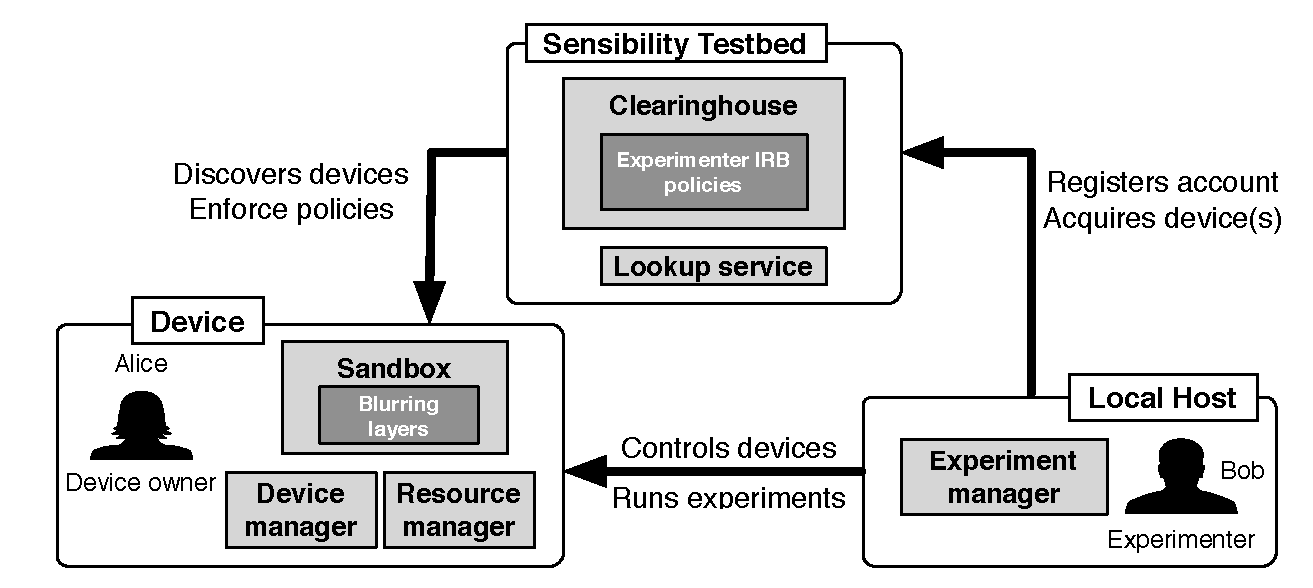
\includegraphics[width=\columnwidth]{figs/arch.pdf}}
%\vspace*{-20pt}
\caption{\small Sensibility Testbed architecture. \label{fig-arch}}
\end{figure}

%\subsubsection{Interacting Parties}\label{sec-parties}
The operation of Sensibility Testbed  involves three types of interacting
parties, as shown in Figure~\ref{fig-arch}: mobile \textit{devices} 
owned by ordinary people, with our app installed; a 
\textit{clearinghouse} server that discovers and configures
participating devices; and \textit{experimenters} who want to run
experiments on mobile devices. The design of \sysname follows
a few guidelines, resulting in the testbed components
shown in Figure~\ref{fig-arch}.
%\subsubsection{Testbed Architecture}

\textbf{Shared access to device resources.} 
Since hardware resources are limited on mobile devices, it is 
not possible to dedicate an entire device to an experiment. Therefore, 
Sensibility Testbed allows several experiments to share one device. It 
uses a \textit{sandbox} to isolate one researcher's code from 
 another, through its performance isolation technique. The sandbox 
also prevents experiment code from inadvertently harming the device
via security isolation. Other software within the device includes a 
\textit{resource manager} that controls a researcher's access to a sandbox 
and allows the device to communicate with the rest of the testbed, 
and a \textit{device manager} that allows the device 
owner to opt in or out of the testbed. Together, they form the
\textit{device software} (Section~\ref{sec-repy}).

\textbf{Allocating devices and mediating data access.}
Sensibility Testbed is designed to provide both enhanced security and 
more efficient management of experimental setup, so another principle 
for the design was a central component that could serve as a a trusted 
intermediary for acquiring and managing device resources. Both tasks 
are delegated to  a server called \textit{clearinghouse}~\cite{ch}. The 
clearinghouse allows researchers to 
register accounts for each experiment, and share access to a common 
pool of devices, freeing them from the need to individually recruit participants. 
The clearinghouse can also allocate resources and mediate 
data access according to policies defined by a researcher's IRB. The 
clearinghouse thus facilitates device sharing and policy enforcement.  
Additionally, the clearinghouse uses a distributed service called 
\textit{lookup service} to keep track of the devices in the testbed 
(Section~\ref{sec-ch}).

\textbf{Local support for remote experimentation.} 
The last design principle was to allow researchers to manage their 
experiments on remote devices from a local machine, as is offered 
by other testbeds~\cite{hibler2008large, peterson2006experiences}. Sensibility 
Testbed addresses this need by using a tool called \textit{experiment 
manager}. The experiment manager provides access to 
hardware resources on mobile devices using the researcher's testbed 
credentials (assigned by the clearinghouse). This tool will be introduced
in Section~\ref{sec-emt}.

%\smallskip
%The following section describes %the three components in more detail, and 
%%addresses 
%how these parties interact to enable safe experimentation on mobile devices. 


